\documentclass{article}
\usepackage{amsmath, amssymb}
\usepackage{listings}
\usepackage{tikz}

\lstset{
  basicstyle=\ttfamily\footnotesize,
  breaklines=true,
  keywordstyle=\bfseries,
  commentstyle=\itshape,
  mathescape=true,
  escapeinside={(*}{*)},
  keepspaces=true,
  morekeywords={data,where,postulate}
}

\begin{document}

\title{Issue XXVIII: Categories with Families}
\author{Namdak Tonpa}
\date{}

\maketitle

\begin{abstract}
We present a categorical model of Martin-Löf Type Theory (MLTT-75) with dependent products ($\Pi$-types), dependent sums ($\Sigma$-types), identity types (Id-types), and additional types ($\top$, U, Bool), formalized in Agda using Categories with Families (CwF) as described in \cite{awodey2019}. The model captures type dependency and context extension via a presheaf of families and context comprehension, supporting all specified type formers. Formal definitions and Agda code are provided, with pullback diagrams resembling Awodey’s natural models, illustrating the type formers with constructors (e.g., $\lambda$, pair, refl) on upper arrows and type formers on lower arrows.
\end{abstract}

\section{Categories with Families}

\subsection{Визначення}

\begin{definition}[Fam]
Категорія $Fam$ --- це категорія сімей множин, де об’єкти є залежними функціональними просторами $(x:A)\rightarrow B(x)$, а морфізми з доменом $\Pi(A,B)$ і кодоменом $\Pi(A',B')$ --- це пари функцій $\langle f:A\rightarrow A', g(x:A):B(x)\rightarrow B'(f(x)) \rangle$.
\end{definition}

\begin{definition}[$\Pi$-похідність]
Для контексту $\Gamma$ і типу $A$ позначимо $\Gamma\vdash A = (\gamma:\Gamma)\rightarrow A(\gamma)$.
\end{definition}

\begin{definition}[$\Sigma$-охоплення]
Для контексту $\Gamma$ і типу $A$ маємо $\Gamma;A = (\gamma:\Gamma)*A(\gamma)$. Охоплення не є асоціативним:
\[
    \Gamma;A;B \neq \Gamma;B;A
\]
\end{definition}

\begin{definition}[Контекст]
Категорія контекстів $C$ --- це категорія, де об’єкти є контекстами, а морфізми --- підстановками. Термінальний об’єкт $\Gamma=0$ у $C$ називається порожнім контекстом. Операція охоплення контексту $\Gamma;A = (x:\Gamma)*A(x)$ має елімінатори: $p:\Gamma;A\vdash\Gamma$, $q:\Gamma;A\vdash A(p)$, що задовольняють універсальну властивість: для будь-якого $\Delta:ob(C)$, морфізму $\gamma:\Delta\rightarrow\Gamma$ і терму $a:\Delta\rightarrow A$ існує єдиний морфізм $\theta=\langle\gamma,a\rangle:\Delta\rightarrow\Gamma;A$, такий що $p\circ\theta=\gamma$ і $q(\theta)=a$. Твердження: підстановка є асоціативною:
\[
    \gamma(\gamma(\Gamma,x,a),y,b) = \gamma(\gamma(\Gamma,y,b),x,a)
\]
\end{definition}

\begin{definition}[CwF-об’єкт]
CwF-об’єкт --- це пара $\Sigma(C, C\rightarrow Fam)$, де $C$ --- категорія контекстів з об’єктами-контекстами та морфізмами-підстановками, а $T:C\rightarrow Fam$ --- функтор, який відображає контекст $\Gamma$ у $C$ на сім’ю множин термів $\Gamma\vdash A$, а підстановку $\gamma:\Delta\rightarrow\Gamma$ --- на пару функцій, що виконують підстановку $\gamma$ у термах і типах відповідно.
\end{definition}

\begin{definition}[CwF-морфізм]
Нехай $(C,T):ob(C)$, де $T:C\rightarrow Fam$. CwF-морфізм $m: (C,T)\rightarrow(C',T')$ --- це пара $\langle F:C\rightarrow C', \sigma:T\rightarrow T'(F) \rangle$, де $F$ --- функтор, а $\sigma$ --- натуральна трансформація.
\end{definition}

\begin{definition}[Категорія типів]
Для CwF з об’єктами $(C,T)$ і морфізмами $(C,T)\rightarrow(C',T')$, для заданого контексту $\Gamma \in Ob(C)$ можна побудувати категорію $Type(\Gamma)$ --- категорію типів у контексті $\Gamma$, де об’єкти --- множина типів у контексті, а морфізми --- функції $f:\Gamma;A\rightarrow B(p)$.
\end{definition}

\subsection{Семантика залежної теорії типів}

\begin{definition}[Терми та типи]
У CwF для контексту $\Gamma$ терми $\Gamma\vdash a:A$ є елементами множини $A(\gamma)$, де $\gamma:\Gamma$. Типи $\Gamma\vdash A$ є об’єктами в $Type(\Gamma)$, а підстановка $\gamma:\Delta\rightarrow\Gamma$ діє на типи та терми через функтор $T$.
\end{definition}

\begin{theorem}[Композиція підстановок]
Підстановки в категорії контекстів $C$ є асоціативними та мають одиницю (ідентичну підстановку). Формально, для $\gamma:\Delta\rightarrow\Gamma$, $\delta:\Theta\rightarrow\Delta$ і $\epsilon:\Gamma\rightarrow\Lambda$ виконується:
\[
    (\gamma \circ \delta) \circ \epsilon = \gamma \circ (\delta \circ \epsilon), \quad id_{\Gamma} \circ \gamma = \gamma, \quad \gamma \circ id_{\Delta} = \gamma.
\]
\end{theorem}

\begin{proof}
Асоціативність випливає з універсальної властивості охоплення контексту (Визначення 1.4). Для будь-яких $\gamma,\delta,\epsilon$ композиція морфізмів у $C$ відповідає послідовному застосуванню підстановок, що зберігає структуру контекстів. Ідентична підстановка $id_{\Gamma}$ діє як нейтральний елемент, оскільки $p \circ id_{\Gamma} = id_{\Gamma}$ і $q(id_{\Gamma}) = q$.
\end{proof}

\begin{definition}[Залежні типи]
Залежний тип у контексті $\Gamma$ --- це відображення $\Gamma \rightarrow Fam$, де для кожного $\gamma:\Gamma$ задається множина $A(\gamma)$. У категорії $Type(\Gamma)$ залежні типи є об’єктами, а морфізми між $A$ і $B$ --- це функції $f: \Gamma;A \rightarrow B(p)$, що зберігають структуру підстановок.
\end{definition}

\begin{theorem}[Універсальна властивість залежних типів]
Для будь-якого контексту $\Gamma$, типу $A$ і терму $a:\Gamma\vdash A$ існує унікальний морфізм $\theta:\Gamma \rightarrow \Gamma;A$, який задовольняє $p \circ \theta = id_{\Gamma}$ і $q(\theta) = a$. Це забезпечує коректність залежної типізації в CwF.
\end{theorem}

\begin{proof}
За Визначенням 1.4, універсальна властивість охоплення контексту гарантує існування $\theta = \langle id_{\Gamma}, a \rangle$. Унікальність випливає з того, що будь-який інший морфізм $\theta'$ з тими ж властивостями ($p \circ \theta' = id_{\Gamma}$, $q(\theta') = a$) збігається з $\theta$ через єдиність композиції в $C$.
\end{proof}

Martin-Löf Type Theory (MLTT-75) is a dependent type theory with $\Pi$-types, $\Sigma$-types, Id-types, and additional type formers like $\top$, universe types (U), and Bool. Its categorical semantics can be modeled using Categories with Families (CwF), a framework designed to capture contexts, types, terms, and context extension in a unified way \cite{awodey2019, ncatlab}. Unlike Grothendieck fibrations or comprehension categories, CwFs use a presheaf of families to represent types and terms, with context comprehension for type dependency. We formalize a CwF model for MLTT-75 in Agda, supporting all specified type formers, based on \cite{awodey2019}. Pullback diagrams, styled after Awodey’s natural models \cite{awodey}, illustrate the type formers, with constructors on upper arrows and type formers on lower arrows.

A Category with Families (CwF) models dependent type theory by assigning types and terms to contexts, with context comprehension for type dependency.

\newpage
\begin{definition}[Category with Families]
A \emph{Category with Families} (CwF) consists of:
\begin{itemize}
  \item A category $\mathcal{C}$ with a terminal object $1 \in \mathcal{C}.\text{Ob}$.
  \item A presheaf $\text{Ty} : \mathcal{C}^{\text{op}} \to \text{Set}$, assigning to each $\Gamma \in \mathcal{C}.\text{Ob}$ a set $\text{Ty}(\Gamma)$ of types, and to each $\sigma : \Delta \to \Gamma$ a function $\sigma^* : \text{Ty}(\Gamma) \to \text{Ty}(\Delta)$, preserving identities and composition.
  \item For each $\Gamma \in \mathcal{C}.\text{Ob}$ and $A \in \text{Ty}(\Gamma)$, a set $\text{Tm}(\Gamma, A)$ of terms, with reindexing: for $\sigma : \Delta \to \Gamma$, a function $\text{Tm}(\Gamma, A) \to \text{Tm}(\Delta, \sigma^* A)$, preserving identities and composition.
  \item For each $\Gamma \in \mathcal{C}.\text{Ob}$ and $A \in \text{Ty}(\Gamma)$, a context comprehension consisting of:
    \begin{itemize}
      \item An object $\Gamma.A \in \mathcal{C}.\text{Ob}$.
      \item A projection morphism $p_A : \Gamma.A \to \Gamma$.
      \item A universal term $q_A \in \text{Tm}(\Gamma.A, p_A^* A)$.
      \item For any $\Delta \in \mathcal{C}.\text{Ob}$, $\sigma : \Delta \to \Gamma$, and $t \in \text{Tm}(\Delta, \sigma^* A)$, there exists a unique $\langle \sigma, t \rangle : \Delta \to \Gamma.A$ such that $p_A \circ \langle \sigma, t \rangle = \sigma$ and $\langle \sigma, t \rangle^* q_A = t$.
    \end{itemize}
\end{itemize}
\end{definition}

\subsection{Type Formers}
To model MLTT-75, the CwF is equipped with structure for $\Pi$-types, $\Sigma$-types, Id-types, $\top$, U, and Bool.

\begin{definition}[CwF with MLTT-75 Type Formers]
A \emph{CwF with MLTT-75 type formers} extends a CwF with:
\begin{itemize}
  \item \emph{Empty context}: An object $\bullet \in \mathcal{C}.\text{Ob}$ with a unique morphism $\epsilon : \Gamma \to \bullet$ for any $\Gamma$.
  \item \emph{Pullbacks}: For any $f : A \to B$, $g : C \to B$ in $\mathcal{C}$, there exists a pullback $P$ with morphisms $h_1 : P \to A$, $h_2 : P \to C$ such that $f \circ h_1 = g \circ h_2$, and $P$ is universal.
  \item \emph{$\Pi$-types}: For $\Gamma \in \mathcal{C}.\text{Ob}$, $A \in \text{Ty}(\Gamma)$, $B \in \text{Ty}(\Gamma.A)$, there exists $\Pi_A B \in \text{Ty}(\Gamma)$, a term $\text{lam}(t) \in \text{Tm}(\Gamma, \Pi_A B)$ for $t \in \text{Tm}(\Gamma.A, B)$, and $\text{app} : \text{Tm}(\Gamma, \Pi_A B) \to \text{Tm}(\Gamma.A, B)$, satisfying $\beta$- and $\eta$-rules.
  \item \emph{$\Sigma$-types}: For $\Gamma \in \mathcal{C}.\text{Ob}$, $A \in \text{Ty}(\Gamma)$, $B \in \text{Ty}(\Gamma.A)$, there exists $\Sigma_A B \in \text{Ty}(\Gamma)$, a term $(u, v) \in \text{Tm}(\Gamma, \Sigma_A B)$ for $u \in \text{Tm}(\Gamma, A)$, $v \in \text{Tm}(\Gamma, B[\text{id}, u])$, and projections $\text{fst}$, $\text{snd}$, satisfying $\beta$- and $\eta$-rules.
  \item \emph{Id-types}: For $\Gamma \in \mathcal{C}.\text{Ob}$, $A \in \text{Ty}(\Gamma)$, $a, b \in \text{Tm}(\Gamma, A)$, there exists $\text{Id}_A(a, b) \in \text{Ty}(\Gamma)$, a term $\text{refl}(u) \in \text{Tm}(\Gamma, \text{Id}_A(u, u))$, and an eliminator $J$, satisfying $\beta$-rule.
\end{itemize}
\end{definition}

\newpage
\begin{lstlisting}[mathescape=true]
def algebra : U₁ := Σ
    -- a semicategory of contexts and substitutions:
    (Con: U)
    (Sub: Con → Con → U)
    (◊: Π (Г Θ ∆ : Con), Sub Θ ∆ → Sub Г Θ → Sub Г ∆)
    (◊-assoc: Π (Г Θ ∆ Ф : Con) (σ: Sub Г Θ) (δ: Sub Θ ∆)
        (ν: Sub ∆ Ф), PathP (<_>Sub Г Ф) (◊ Г ∆ Ф ν (◊ Г Θ ∆ δ σ))
                                         (◊ Г Θ Ф (◊ Θ ∆ Ф ν δ) σ))
    -- identity morphisms as identity substitutions:
    (id: Π (Г : Con), Sub Г Г)
    (id-left: Π (Θ ∆ : Con) (δ : Sub Θ ∆),
              Path (Sub Θ ∆) δ (◊ Θ ∆ ∆ (id ∆) δ))
    (id-right: Π (Θ ∆ : Con) (δ : Sub Θ ∆),
               Path (Sub Θ ∆) δ (◊ Θ Θ ∆ δ (id Θ)))
    -- a terminal oject as empty context:
    (•: Con)
    (є: Π (Г : Con), Sub Г •)
    (•-η: Π (Г: Con) (δ: Sub Г •), Path (Sub Г •) (є Г) δ)
    (Ty: Con → U)
    (_|_|ᵀ: Π (Г ∆ : Con), Ty ∆ → Sub Г ∆ → Ty Г)
    (|id|ᵀ: Π (∆ : Con) (A : Ty ∆), Path (Ty ∆) (_|_|ᵀ ∆ ∆ A (id ∆)) A)
    (|◊|ᵀ: Π (Г ∆ Ф: Con) (A : Ty Ф) (σ : Sub Г ∆) (δ : Sub ∆ Ф),
        PathP (<_>Ty Г) (_|_|ᵀ Г Ф A (◊ Г ∆ Ф δ σ))
                        (_|_|ᵀ Г ∆ (_|_|ᵀ ∆ Ф A δ) σ))
    -- a (covariant) presheaf on the category of elements as terms:
    (Tm: Π (Г : Con), Ty Г → U)
    (_|_|ᵗ: Π (Г ∆ : Con) (A : Ty ∆) (B : Tm ∆ A)
              (σ: Sub Г ∆), Tm Г (_|_|ᵀ Г ∆ A σ))
    (|id|ᵗ: Π (∆ : Con) (A : Ty ∆) (t: Tm ∆ A),
            PathP (<i> Tm ∆ (|id|ᵀ ∆ A @ i))
                  (_|_|ᵗ ∆ ∆ A t (id ∆)) t)
    (|◊|ᵗ: Π (Г ∆ Ф: Con) (A : Ty Ф) (t: Tm Ф A)
             (σ : Sub Г ∆) (δ : Sub ∆ Ф),
             PathP (<i> Tm Г (|◊|ᵀ Г ∆ Ф A σ δ @ i))
                   (_|_|ᵗ Г Ф A t (◊ Г ∆ Ф δ σ))
          (_|_|ᵗ Г ∆ (_|_|ᵀ ∆ Ф A δ) (_|_|ᵗ ∆ Ф A t δ) σ))
\end{lstlisting}

\newpage
\subsection{Example MLTT-75 Model}

We model MLTT-75 using a CwF with type formers, interpreting contexts, types, and terms via the presheaf of families and context comprehension.

\begin{definition}[MLTT-75 CwF Model]
Given a CwF with type formers, the model of MLTT-75 is defined as:
\begin{itemize}
  \item \emph{Contexts}: Objects $\Gamma \in \mathcal{C}.\text{Ob}$, indexed by levels $i \in \mathbb{N}$.
  \item \emph{Types}: Elements $A \in \text{Ty}_i(\Gamma)$, indexed by levels.
  \item \emph{Terms}: Elements $t \in \text{Tm}(\Gamma, A)$.
  \item \emph{Context extension}: For $\Gamma \vdash A$, the context $\Gamma, x : A$ is $\Gamma.A$, with projection $p_A : \Gamma.A \to \Gamma$.
  \item \emph{Type formers}: $\Pi$-types via fiber exponentials, $\Sigma$-types via dependent sums, Id-types via diagonals, $\top$ as the unit type, U as a universe, Bool with case analysis.
\end{itemize}
\end{definition}

\subsection{$\Pi$-Types}
For $\Gamma \vdash A : \text{Type}_i$ and $\Gamma, x : A \vdash B : \text{Type}_j$, the $\Pi$-type $\Pi_{x : A} B : \text{Type}_{i \sqcup j}$ is formed using exponentials in the presheaf category.

The constructor $\lambda$ forms terms of $\Pi_{x : A} B$. The pullback diagram is:

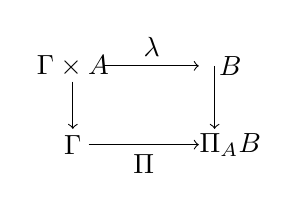
\begin{tikzpicture}
  \node at (0,1) {$\Gamma \times A$};
  \node at (2,1) {$B$};
  \node at (0,0) {$\Gamma$};
  \node at (2,0) {$\Pi_A B$};
  \draw[->] (0.4,1) -- node[above] {$\lambda$} (1.6,1);
  \draw[->] (0,0.8) -- (0,0.2);
  \draw[->] (1.8,1) -- (1.8,0.2);
  \draw[->] (0.2,0) -- node[below] {$\Pi$} (1.6,0);
\end{tikzpicture}

\subsection{$\Sigma$-Types}
For $\Gamma \vdash A : \text{Type}_i$ and $\Gamma, x : A \vdash B : \text{Type}_j$, the $\Sigma$-type $\Sigma_{x : A} B : \text{Type}_{i \sqcup j}$ is formed via dependent sums in the CwF.

The constructor $\text{pair}$ forms terms of $\Sigma_{x : A} B$. The pullback diagram is:

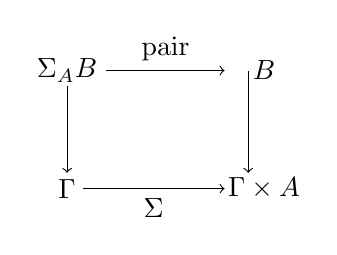
\begin{tikzpicture}
  \node at (0,1.5) {$\Sigma_A B$};
  \node at (2.5,1.5) {$B$};
  \node at (0,0) {$\Gamma$};
  \node at (2.5,0) {$\Gamma \times A$};
  \draw[->] (0.5,1.5) -- node[above] {$\text{pair}$} (2.0,1.5);
  \draw[->] (0,1.3) -- (0,0.2);
  \draw[->] (2.3,1.5) -- (2.3,0.2);
  \draw[->] (0.2,0) -- node[below] {$\Sigma$} (2.0,0);
\end{tikzpicture}

\newpage
\subsection{Id-Types}
For $\Gamma \vdash A : \text{Type}_i$ and $a, b : A$, the identity type $\text{Id}_A(a, b) : \text{Type}_i$ is formed using the diagonal map in the CwF.

The constructor $\text{refl}$ forms terms of $\text{Id}_A(a, a)$. The pullback diagram is:

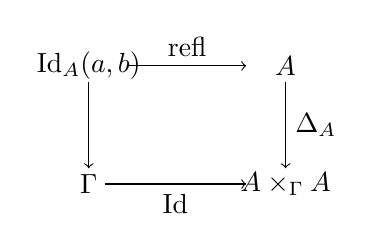
\begin{tikzpicture}
  \node at (0,1.5) {$\text{Id}_A(a, b)$};
  \node at (2.5,1.5) {$A$};
  \node at (0,0) {$\Gamma$};
  \node at (2.5,0) {$A \times_\Gamma A$};
  \draw[->] (0.5,1.5) -- node[above] {$\text{refl}$} (2.0,1.5);
  \draw[->] (0,1.3) -- (0,0.2);
  \draw[->] (2.5,1.3) -- node[right] {$\Delta_A$} (2.5,0.2);
  \draw[->] (0.2,0) -- node[below] {$\text{Id}$} (2.0,0);
\end{tikzpicture}

\subsection{Conclusion}
The Agda formalization provides a categorical semantics for MLTT-75 using a Category with Families, capturing type dependency and context extension via a presheaf of families and context comprehension. Supporting $\Pi$-types, $\Sigma$-types, Id-types, $\top$, U, and Bool, the model, based on \cite{awodey2019}, contrasts with fibration-based approaches by directly encoding types and terms. The pullback diagrams, styled after Awodey, clarify the categorical constructions. Future work includes exploring univalent extensions and concrete instantiations.

\begin{thebibliography}{9}
\bibitem{awodey2019}
Awodey, S., Frey, J., Speight, S., ``Categorical Structures for Type Theory in Univalent Foundations,'' arXiv:1907.07562, 2019.
\bibitem{hofmann1997}
Hofmann, M., ``On the interpretation of type theory in locally cartesian closed categories,'' LFCS, 1997.
\bibitem{jacobs1993}
Jacobs, B., ``Comprehension categories and the semantics of type dependency,'' TCS, 1993.
\bibitem{awodey}
Awodey, S., ``Natural models of homotopy type theory,'' MSCS, 2018.
\end{thebibliography}

\end{document}